% !TeX spellcheck = de_DE

\chapter{Methodologies}
\label{chap:k2}

The following sections introduce the principles of 3D lane marking reconstruction method of this work, with the work flow shown in \cref{fig:FlowChart}.

\cref{sec:LineExtraction} describes the applied standard line detection algorithm for labeling the lane markings. To relate the object coordinates of a point with its image coordinates, \cref{sec:Geometry} introduces the imaging properties of aerial images and their mathematical models, including the collinearity equation and lens distortion correction.

\cref{sec:LineFitting} presents the principle of line fitting and further derives the non-linear \gls{ls} model for line equations in two-point form. With the combination of the extended collinearity equation introduced in \cref{sec:Geometry}, \cref{sec:LSadj} elaborates the usage of line fitting for 3D lane marking reconstruction.% The key challenge is to solve the line fitting problem given weakly-textured environments around lane markings and to solve the quasi-infinite line reconstruction problem.

In \cref{sec:LineProjectionOnDSM} the problem of acquiring initial values is described, as initial values of unknown quantities are required in non-linear LS model. Section2.7??? demonstrates how the corresponding measurements in image space are collected given the initial values in object space.

\begin{figure}
  \centering
  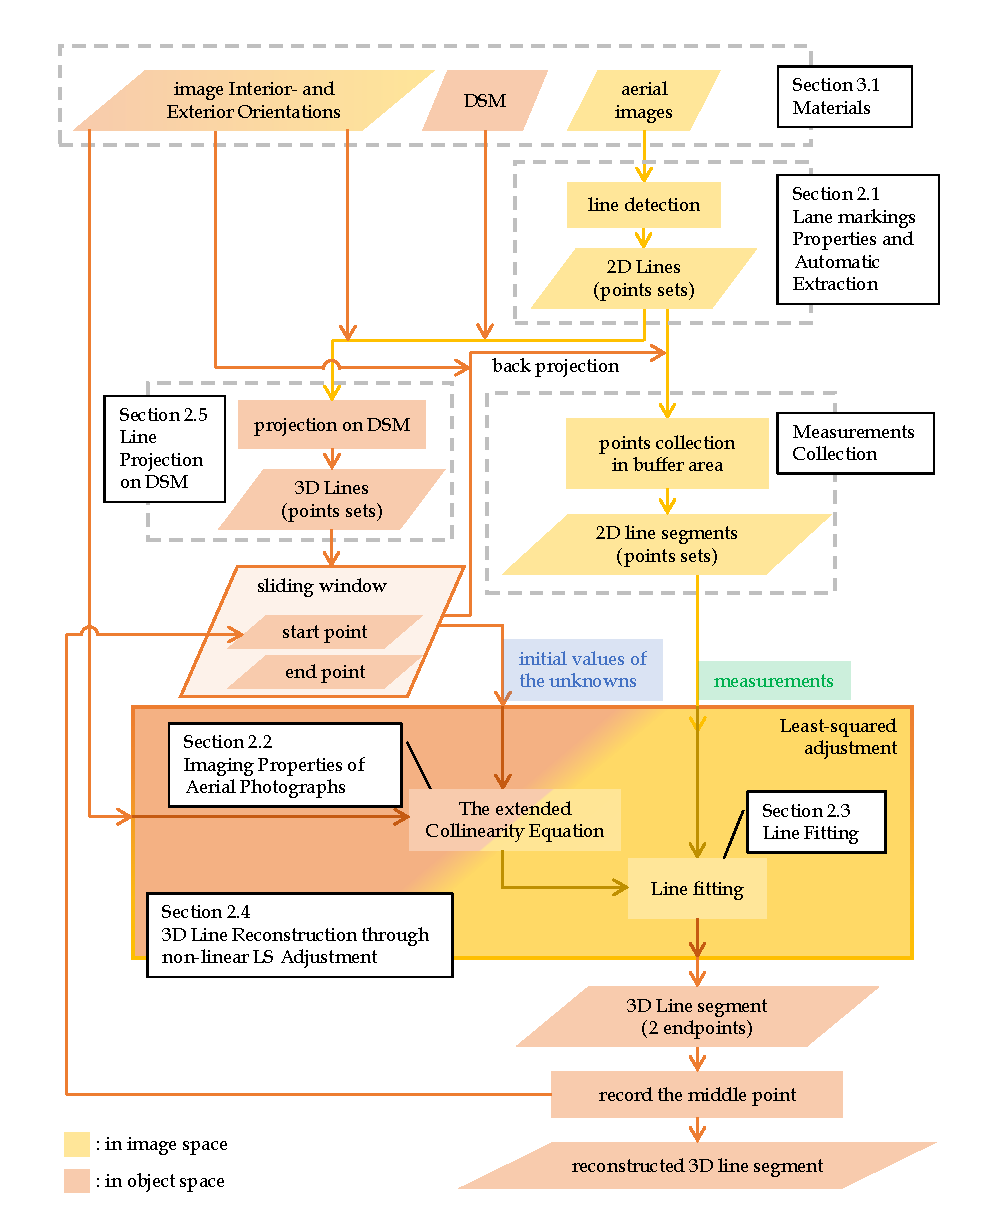
\includegraphics[width=\textwidth]{workflow.pdf}
  \caption{\small The work flow}
  \label{fig:FlowChart}
\end{figure}

\clearpage


%%%%%%%%%%%%%%%%%%%%%%%%%%%%%%%%%%%%%%%%%%%%%%%%%%%%%%%%
\section{Lane markings Properties and Automatic Extraction}
\label{sec:LineExtraction}
% Missing some small review about alternative methods?
% This chapter should be much more detailled.
The appearance of lane markings on German roads including line type, color and width is specified depending on the road type. Different line types of lane markings are shown in \cref{fig:LaneMarkingTypes} and their line widths are defined in \cref{tab:LaneMarkingWidths}. As shown in \cref{tab:DashedLaneMarkingLengths}, the dashed lane markings on motorways are of 6 meter length.
% https://de.wikipedia.org/wiki/Fahrbahnmarkierung#Eigenschaften
% Richtlinien für die Markierung von Straßen (RMS) Teil 1

Because of the appearance, the problem of lane marking detection can be treated as a line detection problem. We restrict the proposed framework to lane markings with single white lines (dashed or continuous) of 0.3 meter width. Other types like in restricted zone, double lines, parking areas, temporal yellow lines in construction sites etc, are excluded.% https://www.transchool.lee.army.mil/adso/documents/zeichen.pdf

The principle to extract line features is to firstly derive the line direction for each pixel by using partial derivatives of a Gaussian smoothing kernel. Pixels that have a local maximum in the second directional derivative perpendicular to the line direction are marked as line points. By thresholding their second directional derivative values, the accepted line points are then linked and connected.
% C. Steger: “Extracting Curvilinear Structures: A Differential Geometric Approach”. In B. Buxton, R. Cipolla, eds., “Fourth European Conference on Computer Vision”, Lecture Notes in Computer Science, Volume 1064, Springer Verlag, pp. 630-641, 1996. 
% C. Steger: “Extraction of Curved Lines from Images”. In “13th International Conference on Pattern Recognition”, Volume II, pp. 251-255, 1996. 
% C. Steger: “An Unbiased Detector of Curvilinear Structures”. IEEE Transactions on Pattern Analysis and Machine Intelligence, vol. 20, no. 2, pp. 113-125, 1998
The resultant connected points which compose a line are of sub-pixel precision. \cref{fig:LineExtraction} shows the extracted lines on the masked original image.
% http://www.mvtec.com/doc/halcon/11/en/lines_gauss.html

\begin{figure}
\centering
\subfloat[\small Continuous line]{\fbox{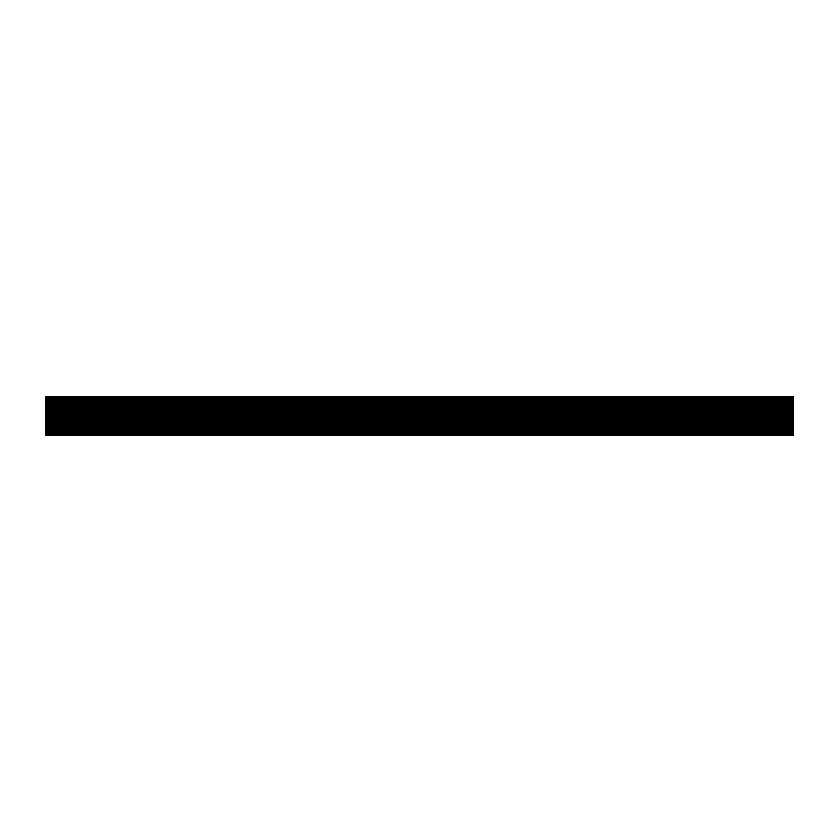
\includegraphics[width=0.3\textwidth, trim={0 150 0 150},clip=true]{Laengsmarkierung_durchgehend.pdf}}}
\quad
\subfloat[\small Dashed line]{\fbox{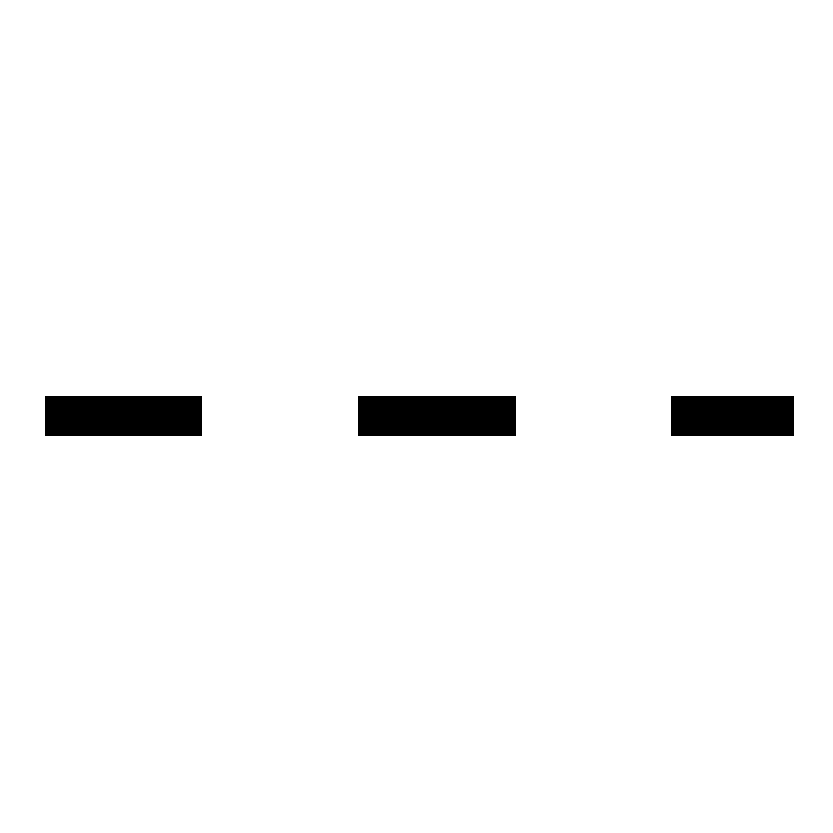
\includegraphics[width=0.3\textwidth, trim={0 150 0 150},clip=true]{Laengsmarkierung_unterbrochen.pdf}}}
\newline
\subfloat[\small Continuous and dashed double lines]{\fbox{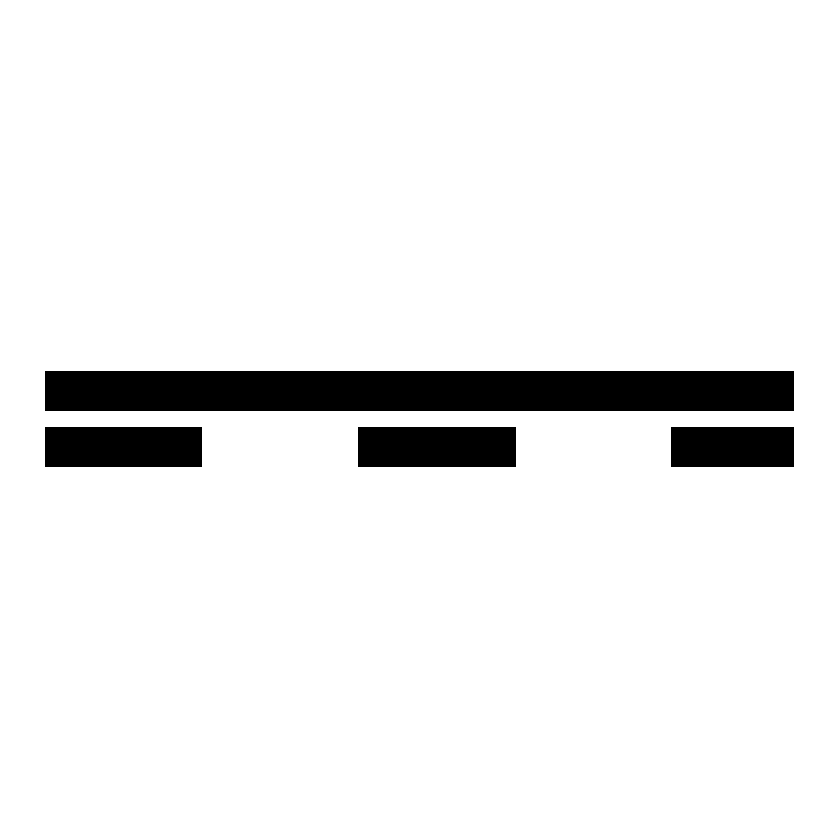
\includegraphics[width=0.3\textwidth, trim={0 150 0 150},clip=true]{Laengsmarkierung_unterbrochen_durchgehend.pdf}}}
\quad
\subfloat[\small Continuous double lines]{\fbox{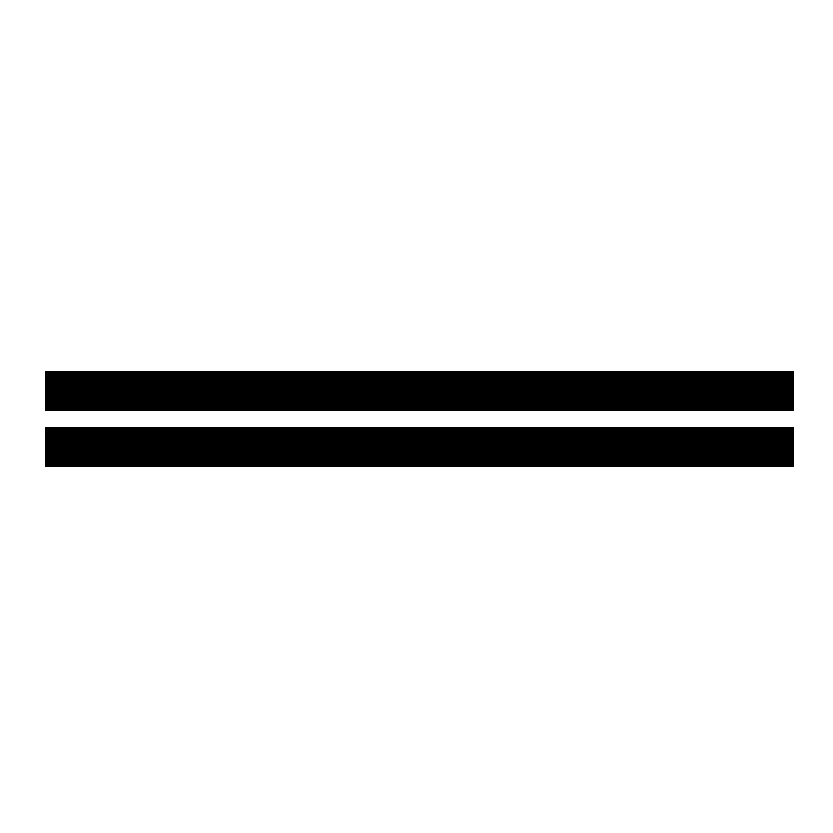
\includegraphics[width=0.3\textwidth, trim={0 150 0 150},clip=true]{Laengsmarkierung_durchgehend_doppelt.pdf}}}
\quad
\subfloat[\small Dashed double lines]{\fbox{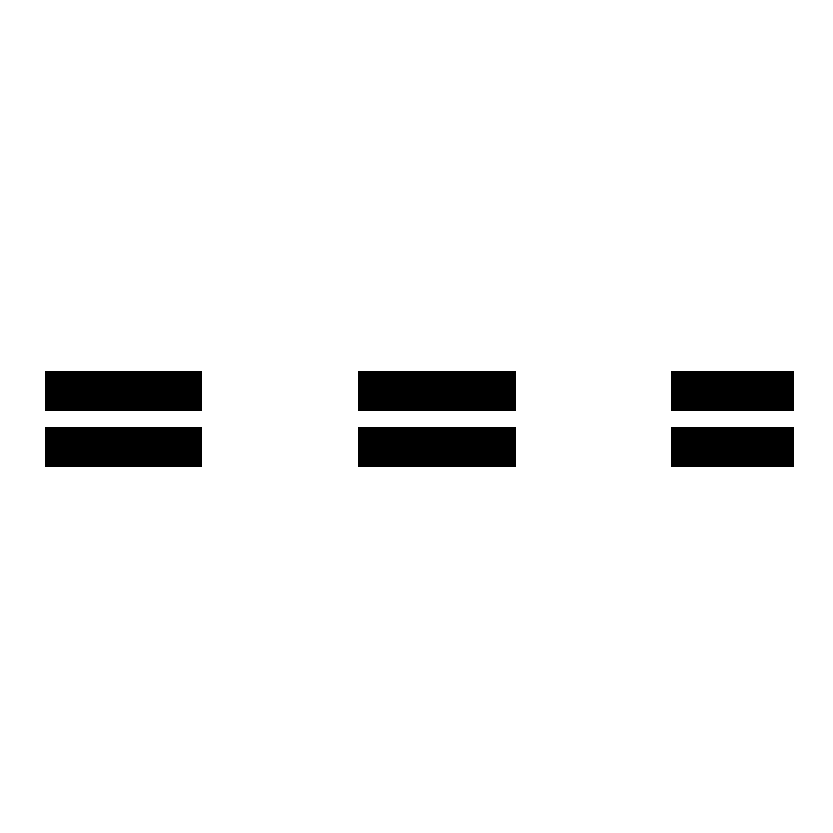
\includegraphics[width=0.3\textwidth, trim={0 150 0 150},clip=true]{Laengsmarkierung_unterbrochen_doppelt.pdf}}}
\caption{\small Line types of lane markings [source RMS Teil 1]}
% https://de.wikipedia.org/wiki/Fahrbahnmarkierung
% Richtlinien für die Markierung von Straßen (RMS) Teil 1
\label{fig:LaneMarkingTypes}
\end{figure}
\setlength{\floatsep}{16pt plus 1.0pt minus 2.0pt}
\begin{table}
    \centering
    \begin{tabular}{l|cc}
    \toprule
           & motorways\footnote{and corresponding roads in the sense of the VwV-StVO to § 42 to mark 330 (motorway) II}  & other roads\\
    \midrule
    narrow lines & $0.15$ [m] & $0.12$ [m] \\
    wide lines   & $0.30$ [m] & $0.25$ [m] \\
    \bottomrule
    \end{tabular}
    \caption{\small Widths of lane markings [source RMS Teil 1]}
    \label{tab:LaneMarkingWidths}
% Der Deutsche Verkehrssicherheitsrat
% https://www.dvr.de/download/publikationen-schriftenreihe-17.pdf
% Richtlinien für die Markierung von Straßen (RMS) Teil 1
\end{table}
\setlength{\floatsep}{16pt plus 1.0pt minus 2.0pt}
\begin{table}
    \centering
    \begin{tabular}{l|ccc}
    \toprule
          & motorways & \multicolumn{2}{c}{other roads}\\
          &           & in town & out of town\\
    \midrule
    line / gap  & $6$ [m] / $12$ [m] & $3$ [m] / $6$ [m] & $4$ [m] / $8$ [m]\\
    \bottomrule
    \end{tabular}
    \caption{\small Lengths of dashed lane markings with ratio 1:2 [source RMS Teil 1]}
    \label{tab:DashedLaneMarkingLengths}
% Der Deutsche Verkehrssicherheitsrat
% https://www.dvr.de/download/publikationen-schriftenreihe-17.pdf
% Richtlinien für die Markierung von Straßen (RMS) Teil 1
\end{table}

\begin{figure}
  \centering
  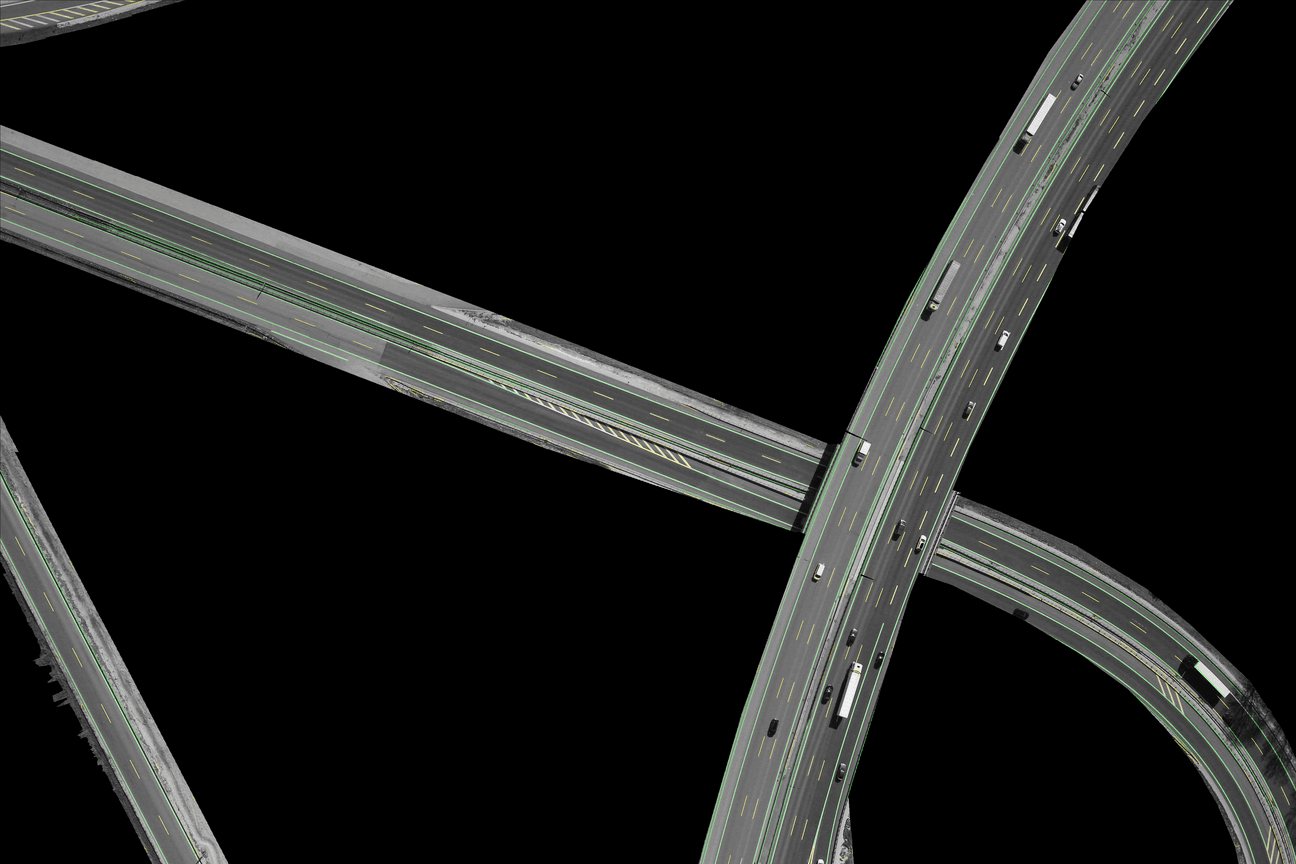
\includegraphics[width=0.7\textwidth, trim=750 250 200 320,clip]{ML1234_extlines_rsz.png}
  \caption{\small Lane markings Extraction. The extracted long lane-lines are marked in green and the dashed ones are in yellow.  Note that both cases are reconstructed into 3D with the same framework; different colors here are only for illustration.}
  \label{fig:LineExtraction}
\end{figure}



%%%%%%%%%%%%%%%%%%%%%%%%%%%%%%%%%%%%%%%%%%%%%%%%%%%%%%%%
\section{Imaging Properties of Aerial Photographs}
\label{sec:Geometry}

This section describes the geometric model of the projection of 3D points into the image generated by a real camera. We first restrict the discussion in \cref{subsec:Collinearity} to central perspective projection where the collinearity equation originate from. We then model deviations from this model, addressing real cameras with imperfect lenses, in \cref{subsec:LensDistortion}.

\subsection{Collinearity Equations}
\label{subsec:Collinearity}
We assume frame photography, i.e. photographs exposed on a frame chip in one instant, and assume central projection model with cameras that have a single viewpoint and a planar sensor and being straight line-preserving. Collinearity indicates the condition that the image point (on the sensor plate of the camera), the observed point (in object space) and the projection center of the camera were aligned at the moment the picture was taken. Every measured point leads to two collinearity equations, describing transformations from object space to image coordinates:
\begin{equation} \label{eq:collinearity}
\begin{split}
x = x_0 -c \dfrac {R_{11}(X-X_0) + R_{21}(Y-Y_0) + R_{31}(Z-Z_0)} {R_{13}(X-X_0) + R_{23}(Y-Y_0) + R_{33}(Z-Z_0)} \\
y = y_0 -c \dfrac {R_{12}(X-X_0) + R_{22}(Y-Y_0) + R_{32}(Z-Z_0)} {R_{13}(X-X_0) + R_{23}(Y-Y_0) + R_{33}(Z-Z_0)}
\end{split}
\end{equation}
where\newline
$(x, y)$: image coordinates of the point \newline
$(x_0, y_0)$: image coordinates of principal point \newline
$c$: principal distance; focal length \newline
$(X, Y, Z)$: object coordinates of the point \newline
$(X_0, Y_0, Z_0)$: object coordinates of projection center \newline
$R_{11},...,R_{33}$: elements of the rotation matrix R (orthogonal 3$\times$3-matrix from object space to image space, with 3 independent angles $\omega$, $\phi$ and $\kappa$)

\subsection{Lens Distortion Correction}
\label{subsec:LensDistortion}

An original image appears to have some degree of deviations from perspective mapping due to lens distortion, lens refraction or non-planarity of the sensor surface. There are several models to describe these perturbing effects and can be used to undistort the images, resulting in rectified images which are now straight line-preserving.
 
A subset of physical distortion model [Fraser 1997] is chosen, with two radial symmetric distortion parameters $A_1$ and $A_2$, two asymmetric parameters $B_1$ and $B_2$, and a scaling $C1$ and an affine shearing parameter $C_2$. Assuming $x$ and $y$ to be the distorted image coordinates, the corrections $\Delta x$ and $\Delta y$ are then calculated by the following equations:
\begin{equation} \label{eq:LensDistortion}
\begin{split}
\Delta x &= x_p + A_1x_*(r^2-R_0^2) + A_2x_*(r^4-R_0^4) + B_1(r^2+2x_*^2) + B_22x_*y+C_2y \\
\Delta y &= y_p + A_1y  (r^2-R_0^2) + A_2y  (r^4-R_0^4) + B_1(r^2+2y^2)   + B_22x_*y
\end{split}
\end{equation}
with $r=\sqrt{x_*^2+y^2}$, $x_*=\dfrac{x}{C_1}$ and radius\footnote{At the radius $R_0$ the radial symmetric distortion is zero by definition, which avoids too high distortion values at the edges and reduces the correlation with the focal length.} $R_0$ being set %to 0.014m which corresponds 
to a third of the sensor diagonal.

The undistorted image coordinates $x\prime$ and $y\prime$ are then calculated by
\begin{equation} \label{eq:undistortedimgcoord}
\begin{split}
x\prime=x+\Delta x \\
y\prime=y+\Delta y
\end{split}
\end{equation}

\subsection{Extended Collinearity Equation}
\label{subsec:ExtendedCollinearity}
As real cameras generally only approximate the perspective camera model, lens distortion correction can be additionally included in the collinearity model, attempting to correct the pixel position so that they obey the perspective model with sufficient accuracy.[W. Förstner et al. 2016]% The reference is not the original one

By inserting \eqref{eq:collinearity} and \eqref{eq:LensDistortion} into \eqref{eq:undistortedimgcoord} , the relationship between a 3D point $\mathbf{P}(X, Y, Z)$ and its corresponding distorted image coordinates $\mathbf{p}(x,y)$ can be described as
\begin{equation} \label{eq:expandedcollinearity}
\begin{split}
x =& x_0-c\dfrac{R_{11}(X-X_0)+R_{21}(Y-Y_0)+R_{31}(Z-Z_0)}{R_{13}(X-X_0)+R_{23}(Y-Y_0)+R_{33}(Z-Z_0)} \\
&-(x_p + A_1x_*(r^2-R_0^2) + A_2x_*(r^4-R_0^4) + B_1(r^2+2x_*^2) + B_22x_*y+C_2y)\\
y =& y_0-c\dfrac{R_{12}(X-X_0)+R_{22}(Y-Y_0)+R_{32}(Z-Z_0)}{R_{13}(X-X_0)+R_{23}(Y-Y_0)+R_{33}(Z-Z_0)} \\
&-(y_p + A_1y  (r^2-R_0^2) + A_2y  (r^4-R_0^4) + B_1(r^2+2y^2)   + B_22x_*y)
\end{split}
\end{equation}

To express \eqref{eq:expandedcollinearity} shortly, a function $\mathcal{G}$ is defined as
\begin{equation} \label{eq:Gfunction}
\mathbf{p} = \mathcal{G}(\mathbf{q},\mathbf{P}) 
\end{equation}

which takes the interior and exterior orientations as well as the lens distortion parameters of a camera $\mathbf{q}(x_0,y_0,c,X_0,Y_0,Z_0,R_{11},...,R_{33},A_1,A_2,B_1,B_2,C_1,C_2)$ and the position of a 3D point $\mathbf{P}(X, Y, Z)$, and returns the corresponding distorted image coordinates $\mathbf{p}(x,y)$.


%%%%%%%%%%%%%%%%%%%%%%%%%%%%%%%%%%%%%%%%%%%%%%%%%%%%%%%%
\section{Line Fitting}
\label{sec:LineFitting}

Line fitting is the process of constructing a infinite straight line that has a best fit to a 2D dataset. One of the approaches is linear regression which attempts to find the linear function that "best" predicts the dependent variable values as a function of the independent variable. In this work, "best" predict will be understood as in the \gls{ls} approach: minimization of the sum of squared residuals (differences between the measured and the estimated values of the dependent variable).

In the case of standard linear regression, the regressor $y$ is assumed error free, inconsistencies\footnote{The word "inconsistencies" indicates the unobserved random errors, also called as measurement errors.} are only for the dependent variable $x$. Geometrically it means that the horizontal distances from observed data to the fitted line is minimized. To minimize the perpendicular distances from the data points to the regression line, a orthogonal regression model is derived in \cref{subsec:OrthogonalRegression}.

For a later combination with point-wise extended collinearity equation \eqref{eq:Gfunction} in next section, we aim to fit the line equation in two-point form to the observed dataset. 
% extracted lines produced in \cref{sec:LineExtraction} (in forms of sets of points in image coordinates). 
For such non-linear least squares fitting purpose, a non-linear mixed model is derived in \cref{subsec:NonLinear}. % !!!!!!!!!!!!!!!!!

A functional model is unsolvable when the assumed "dependent" variable is indeed not a function of the independent variables, i.e. the assumed functional relationship does not really exist. Take an observed set of 2D points with their Cartesian coordinates $\{x_i,y_i\}^n_{i=1}$ on a vertical line $x=constant$ for example. Their $y$ values have no dependency on their $x$ values, i.e. knowledge of $x$ tells nothing about $y$. Therefore, for this dataset, the functional model $y=f(x)$ is barely solvable. In such cases, however, $x$ is a function of $y$ (which is actually a constant function) and the equation system which models the dependent variable $x$ being a function of the independent variable $y$ becomes solvable. Regarding the dataset used in this work (which will be described with more details in \cref{sec:Materials}) where the observed 2D points scatter mainly in column direction in image space, the linear relationship between $x$ and $y$ values will be setup as $x=f(y)$ to avoid weakly solvable equations system.


%\subsection{Simple Linear Regression}
%\label{subsec:LinearRegression}

%A simple linear regression model describes the linear relationship between a dependent variable and a regressors (an independent variable). By assuming the regressor $y$ being exactly measured without errors, it accounts only for errors $e_x$ in the dependent variable $x$.

%Given a dataset $\{x_i,y_i\}^n_{i=1}$ of $n$ points on a 2D plane, the model takes the form:
%\begin{equation} \label{eq:SimpleLinearRegression}
%x_i - e_{x_i} = a_0 + a_1y_i
%\end{equation}
%where the regression coefficients $a_0$ and $a_1$ are the unknown parameters to be estimated; the error variable $e_x$ is an unobserved random variable that adds noise to the linear relationship between the dependent variable $x$ and regressor $y$.
%https://en.wikipedia.org/wiki/Linear_regression#Assumptions


\subsection{Orthogonal Regression}
\label{subsec:OrthogonalRegression}
A linear regression model describes a dependent variable as a linear function of the regressor (an independent variable). Given a dataset $\{x_i,y_i\}^n_{i=1}$ of $n$ points on a 2D plane, in the case when both dependent variable $x_i$ and regressor $y_i$ are measured with errors %$e_x$ and $e_y$
, a linear regression model takes the form:
\begin{equation} \label{eq:MixModel1-1}
x_i - e_{x_i} = %a_0 + a_1(y_i-e_{y_i}) = 
a_0 + a_1\bar{y_i}
\end{equation}
where the regression coefficients $a_0$ and $a_1$ are the unknown parameters to be estimated, $\bar{y_i}$ denotes the true but unobserved regressor, and the error variable $e_{x_i}$ is an unobserved random variable that adds noise to the linear relationship between the dependent variable $x$ and true regressor $\bar{y_i}$. The true regressor $\bar{y_i}$ is observed with an error $e_{y_i}$ in the pseudo observation equation:
\begin{equation} \label{eq:MixModel1-2}
y_i-e_{y_i} = \bar{y_i}
\end{equation}
Such models, as the combination of \eqref{eq:MixModel1-1} and \eqref{eq:MixModel1-2}, that account the measurement errors in both dependent variable and regressor, are errors-in-variables models. Further more, for the case of equal error variances, i.e. when $\delta=\dfrac{\sigma_{e_x}}{\sigma_{e_y}}=1$, it is a orthogonal regression model which minimizes the %sum of squared 
perpendicular distances from the data points to the regression line.

% !!!
%As \eqref{eq:MixModel1-1} describes the relationship between observations and unknowns and \eqref{eq:MixModel1-2} describes the relationship between observations, this model is known as the mixed model or Gauss-Helmert model.
% It will be helpful to write the basic equations of the model.

\subsection{Orthogonal Regression in Two-point Form}
\label{subsec:NonLinear}

The two-point form of a infinite line in the Cartesian plane passing through the points $(x_1,y_1)$ and $(x_2,y_2)$ is given by:
\begin{equation} \label{eq:LineInTwoPointForm}
(x-x_1) = \dfrac{(x_2-x_1)}{(y_2-y_1)}\times y-y_1
\end{equation}
with $y_2\neq y_1$, where $(x,y)$ is any point on the line.

Let the unknown coordinates of two different points on a line in 2D space be $(x_1,y_1)$ and $(x_2,y_2)$ and the observed 2D points be $\{x_i,y_i\}^n_{i=1}$ with measurement errors $e_{x_i}$ and $e_{y_i}$ in both variables. The orthogonal regression model in two-point form: 
\begin{equation} \label{eq:MixModel2-1}
x_i - e_{x_i}= (x_1-\dfrac{(x_2-x_1)}{(y_2-y_1)}\times y_1) + \dfrac{(x_2-x_1)}{(y_2-y_1)}\times \bar{y_i}
\end{equation}
\begin{equation} \tag{\ref{eq:MixModel1-2} revisited}
y_i-e_{y_i} = \bar{y_i}
\end{equation}

To express \eqref{eq:MixModel2-1} and \eqref{eq:MixModel1-2} shortly, a function $\mathcal{F}$ is defined as

\begin{equation} \label{eq:Ffunction}
\hat{\mathbf{p}} = \mathcal{F}(\mathbf{p}_s,\mathbf{p}_e,y)
\end{equation}

which takes 2D coordinates of a start-point $\mathbf{p_s}(x_s,y_s)$ and an end-point $\mathbf{p_e}(x_e,y_e)$ that define an infinite line, and takes the measured y-coordinate $y$ of an image point $\mathbf{p}(x,y)$, and returns the estimated image coordinates $\mathbf{\hat{p}}(\hat{x},\hat{y})$ which lies on the infinite line $\overline{\mathbf{p_s}\mathbf{p_s}}$.

Note that as a combination of \eqref{eq:MixModel2-1} and \eqref{eq:MixModel1-2}, function $\mathcal{F}$ is actually composed of
\begin{equation} \label{eq:Ffunction_xy}
\begin{split}
\hat{x} = \mathcal{F}^x(\mathbf{p}_s,\mathbf{p}_e,y)\\
\hat{y} = \mathcal{F}^y(\mathbf{p}_s,\mathbf{p}_e,y)
\end{split}
\end{equation}

%%%%%%%%%%%%%%%%%%%%%%%%%%%%%%%%%%%%%%%%%%%%%%%%%%%%%%%%
\section{3D line reconstruction through non-linear LS Adjustment}
\label{sec:LSadj}

In this section, I describe the process of refining the position of a 3D line segment in the object space so that its back-projection in each image has a best-fit to the extracted line in the image space. To simplify the problem, a lane-marking-segment is partially reconstructed through a sliding window in the object space. Each segment is approximated by a straight line, taking into account the maximum curvature of the highway. 
The length of the sliding window depends on the expected curvature, and for motorways it was fixed to 9m …
% What about dashed lane markings in the middle? Why do you choose 9m -> compromise between robustness and minimized systematic errors.

In the sliding window, a line segment is reconstructed taking into account all the measurements (the detected lines) collected in the corresponding regions in all covering images. Only the middle point of the sliding window is then reconstructed by the least-squares estimator (see chapter xx) %!!!
and is recorded. The sliding window then moves half length forward, and the process of 3D reconstruction started again from the recorded middle point of the previous line segment. Another line segment is then reconstructed, with its middle point being recorded. These recorded middle points are in the end the nodes of the reconstructed line. The reconsideration in overlapping region makes the reconstruction more robust.
% Maybe make figure to illustrate

In \cref{subsec:ObsEqua} I firstly set up a model of observation equations. They describe the fitting of a straight line to the measurements in each covering image, where the fitting lines on different images are transformed from a single 3D straight line segment through the extended collinearity equation \eqref{eq:expandedcollinearity}.

Regarding the fact that the collinearity is a point-wise condition, a line segment is represented by its two endpoints whose object coordinates are the six unknown parameters % First mentioned here, what are the six unknowns?
in the LS model. % Which one? 
Correspondingly, the observation equations are line equations in two-point form. A line equation has however a mathematical meaning of infinite length. Therefore, some constraints on unknowns are necessary to avoid arbitrary locations of the two points on the infinite reconstructed 3D line. The constraint equations are modeled in \cref{subsec:ConEqua}.


% the measurements are collected accordingly.

\subsection{The Gauss-Markov Model with Constraints}
\label{GaussMarkovModelwithConstraints}

\paragraph{The Functional Model}
The Gauss-Markov model with constraints starts from $N$ observations $l_n$ for $U$ unknown parameters $x_u$ with $H$ constraints $h_h$ between the unknowns:
\begin{equation} \label{eq:GM-ObsEq}
\boldsymbol l+\widehat{\boldsymbol v}=\boldsymbol f(\widehat{\boldsymbol x})\quad \textnormal{or}\quad \widehat{\boldsymbol l}=\boldsymbol f(\widehat{\boldsymbol x})
\end{equation}
\begin{equation} \label{eq:GM-ConEq}
\boldsymbol h(\widehat{\boldsymbol x})=\mathbf{0}
\end{equation}

The linearized Gauss-Markov model with constraints between the unknowns is:
\begin{equation} \label{eq:GM-ObsEq-linear}
\widehat{\Delta\boldsymbol l}=\Delta\boldsymbol l+\widehat{\boldsymbol v}=\mathsf{A}\,\widehat{\Delta\boldsymbol x}
\end{equation}
\begin{equation} \label{eq:GM-ConEq-linear}
-\boldsymbol h(\widehat{\boldsymbol x}^a)=\mathsf{H^T}\widehat{\Delta\boldsymbol x}
\end{equation}
with
\begin{equation} \label{eq:GM-ObsEq-linear-l}
\Delta\boldsymbol l=\boldsymbol l-\boldsymbol f(\widehat{\boldsymbol x}^a)
\end{equation}
\begin{equation} \label{eq:GM-ObsEq-linear-x}
\widehat{\Delta\boldsymbol x}=\widehat{\boldsymbol x}-\widehat{\boldsymbol x}^a
\end{equation}

\paragraph{The Stochastic Model}




\subsection{Model of Observation Equations}
\label{subsec:ObsEqua}
% % %
% which can be further rewritten:
%Taylor expansion...(local linear approximation)
%the linear equation can also be expanded

Given a start-point $\mathbf{P}_s(X_s,Y_s,Z_s)$ and an end-point $\mathbf{P}_e(X_e,Y_e,Z_e)$ of a line segment $L$ in the object space and the camera parameters $\mathbf{q}^j$ of camera $j$. Consider the case where there are $J$ images covering this line segment. With the expanded collinearity model \eqref{eq:expandedcollinearity}, the start- and end-points of this line segment's back-projection in image $j$ have the image coordinates $\mathbf{p}^j_s(x^j_s,y^j_s)$ and $\mathbf{p}^j_e(x^j_e,y^j_e)$:
\begin{equation} \label{eq:obsmodel-collinearity}
\begin{split}
\mathbf{p}^j_s = \mathcal{G}(\mathbf{q}^j,\mathbf{P}_s)\\
\mathbf{p}^j_e = \mathcal{G}(\mathbf{q}^j,\mathbf{P}_e)
\end{split}
\qquad
\begin{split}
\forall j=1,2,...J
\end{split}
\end{equation}

%%%%%%%%%%%%%%% !!!!!!!!!!!!!!!!!! %%%%%%%%%%%%%%%%
%Let $l^j$ be the corresponding line segment of $L$ being extracted (observed) on image $j$. Given a dataset $\{x^j_{l,i},y^j_{l,i}\}^{N^j_l}_{i=1}$ of $N^j_l$ points on line segment $l^j$. Rewriting the orthogonal regression model \cref{eq:MixModel2-1} and \cref{eq:MixModel1-2} in the structure of the Gauss-Markov model gives the observation equations in vector form:

%\begin{equation} \label{eq:Ffunction}
%\mathbf{l}+\hat{\mathbf{v}}=\mathbf{f}(\hat{\mathbf{x}}):\quad
%\begin{bmatrix}
% x^j_{l,i} + \hat{e}_{x^j_{l,i}}\\[0.3em]
% y^j_{l,i} + \hat{e}_{y^j_{l,i}}\\[0.3em]
%\end{bmatrix}
%=
%\begin{bmatrix}
%(\hat{x}^j_s-\dfrac{(\hat{x}^j_e-\hat{x}^j_s)}{(\hat{y}^j_e-\hat{y}^j_s)}\times \hat{y}^j_s) + \dfrac{(\hat{x}^j_e-\hat{x}^j_s)}{(\hat{y}^j_e-\hat{y}^j_s)}\times \hat{\bar{y}}_{l,i}\\
%\hat{\bar{y}}_{l,i}
%\end{bmatrix}
%\end{equation}
%which estimates a start-point $\mathbf{p_s}(x_s,y_s)$ and an end-point $\mathbf{p_e}(x_e,y_e)$ that define a infinite line in image space so that the observed image coordinates $\hat{\mathbf{p}}^j_{l,i}(\hat{x}^j_{l,i},\hat{y}^j_{l,i})$ on defined by . % !!!!!!!!!!!!!!!!!


%%%%%%%%%%%%%%% !!!!!!!!!!!!!!!!!! %%%%%%%%%%%%%%%%

Let $l^j$ be the corresponding line segment of $L$ being extracted (observed) on image $j$. Given a dataset $\{x^j_{l,i},y^j_{l,i}\}^{N^j_l}_{i=1}$ of $N^j_l$ points on line segment $l^j$, their estimated image coordinates $\hat{\mathbf{p}}^j_{l,i}(\hat{x}^j_{l,i},\hat{y}^j_{l,i})$ on the infinite line $\overline{\mathbf{p}^j_s,\mathbf{p}^j_e}$ computed from the orthogonal regression model \eqref{eq:Ffunction} are:
\begin{equation} \label{eq:obsmodel-linefitting}
\hat{\mathbf{p}}^j_{l,i} = \mathcal{F}(\mathbf{p}^j_s,\mathbf{p}^j_e,y^j_{l,i})
\qquad
\forall i=1,2,...N^j_l
\end{equation}
%%%%%%%%%%%%%%%

Combining \eqref{eq:obsmodel-collinearity} with \eqref{eq:obsmodel-linefitting} gives function $\mathcal{H}$:
\begin{equation} \label{eq:obsmodel}
\begin{split}
\hat{\mathbf{p}}^j_{l,i} &= \mathcal{F}(\mathcal{G}(\mathbf{q}^j,\mathbf{P}_s),\mathcal{G}(\mathbf{q}^j,\mathbf{P}_e),y^j_{l,i})\\
&=\mathcal{H}(\mathbf{q}^j,\mathbf{P}_s,\mathbf{P}_e,y^j_{l,i})
\qquad
\forall i=1,2,...N^j_l,\quad\forall j=1,2,...J
\end{split}
\end{equation}
which takes camera parameters $\mathbf{q}^j(x_0,y_0,c,X_0,Y_0,Z_0,R_{11},...,R_{33},A_1,A_2,B_1,B_2,C_1,C_2)$, object coordinates of $\mathbf{P}_s$ and $\mathbf{P}_e$ which define a line $\overline{\mathbf{P}_s,\mathbf{P}_e}$, and the observed y-coordinate of the point $\mathbf{p}^j_{l,i}$ in image space, and returns the estimated image coordinates $\hat{\mathbf{p}}^j_{l,i}$ on the back projected line of $\overline{\mathbf{P}_s,\mathbf{P}_e}$.
%In \cref{eq:obsmodel}, $y^j_{l,i}, i=1,2,...N^j_l$ are the measurements, $P_s$ and $P_e$ are the unknown quantities, $\mathbf{q}^j, j=1,2,...J$ includes  interior and exterior orientations as well as the lens distortion parameters of camera $j$.\newline

Corresponding to \cref{eq:Ffunction_xy}, function $\mathcal{H}$ is composed of
\begin{equation} \label{eq:obsmodel2}
\begin{split}
\hat{x}^j_{l,i} = \mathcal{H}^x(\mathbf{q}^j,\mathbf{P}_s,\mathbf{P}_e,y^j_{l,i})\\
\hat{y}^j_{l,i} = \mathcal{H}^y(\mathbf{q}^j,\mathbf{P}_s,\mathbf{P}_e,y^j_{l,i})
\end{split}
\qquad
\begin{split}
\forall i=1,2,...N^j_l,\quad\forall j=1,2,...J
\end{split}
\end{equation}

Since the adjustment will be done "segment-wise"--- for a pair of $P_s$ and $P_e$, the measurements will be collected correspondingly. % see section ???
Thus the subscription $l$ representing specific line segment will be left out in the followings.

\clearpage
Each image gives $2\times N^j$ observation equations\footnote{Dot equal indicates inconsistencies between the measured values, $x^j_i$ and $x^j_i$, and the computed values, $\mathcal{H}^x(q^j,P_s,P_e,y^j_i)$ and $\mathcal{H}^y(q^j,P_s,P_e,y^j_i)$.}. These equations are often stacked together and written in vector form as:
\begin{equation} \label{eq:Ffunction}
\begin{bmatrix}
 x^j_1\\[0.3em]
 x^j_2\\[0.3em]
 \vdots\\[0.3em]
 x^j_{N^j}\\[0.5em]
 \arrayrulecolor{lightgray} \hline
 y^j_1\\[0.3em]
 y^j_2\\[0.3em]
 \vdots\\[0.3em]
 y^j_{N^j}\\[0.5em]
\end{bmatrix}
\doteq
\begin{bmatrix}
 \mathcal{H}^x(\mathbf{q}^j,\hat{\mathbf{P}}_s,\hat{\mathbf{P}}_e,y^j_{1})\\[0.3em]
 \mathcal{H}^x(\mathbf{q}^j,\hat{\mathbf{P}}_s,\hat{\mathbf{P}}_e,y^j_{2})\\[0.3em]
 \vdots\\[0.3em]
 \mathcal{H}^x(\mathbf{q}^j,\hat{\mathbf{P}}_s,\hat{\mathbf{P}}_e,y^j_{N^j})\\[0.5em]
 \arrayrulecolor{lightgray} \hline
 \mathcal{H}^y(\mathbf{q}^j,\hat{\mathbf{P}}_s,\hat{\mathbf{P}}_e,y^j_{1})\\[0.3em]
 \mathcal{H}^y(\mathbf{q}^j,\hat{\mathbf{P}}_s,\hat{\mathbf{P}}_e,y^j_{2})\\[0.3em]
 \vdots\\[0.3em]
 \mathcal{H}^y(\mathbf{q}^j,\hat{\mathbf{P}}_s,\hat{\mathbf{P}}_e,y^j_{N^j})\\[0.5em]
\end{bmatrix}
\begin{array}{@{\kern-\nulldelimiterspace}l@{}}
 \left.\begin{array}{@{}c@{}}\\[0.3em] \\[0.3em] \\[0.3em] \\[0.5em] \end{array}\right\} N^j\\
 \left.\begin{array}{@{}c@{}}\\[0.3em] \\[0.3em] \\[0.3em] \\[0.5em] \end{array}\right\} N^j\\
\end{array}
\end{equation}

For all covering image $j=1,2,...J$, there are $2\times\displaystyle\sum_{j=1}^{J}N^j$ observation equations. Being written in the structure of the Gauss-Markov model with constraints, corresponding to \cref{eq:GM-ObsEq}, they are expressed as:
\begin{equation} \label{eq:obsvec-allcam}
\boldsymbol l+\widehat{\boldsymbol v}=\boldsymbol f(\widehat{\boldsymbol x}):\quad
\begin{bmatrix}
 x^1_1\\[0.3em]
 \vdots\\
 x^1_{N^1}\\[0.3em]
 \arrayrulecolor{lightgray} \hline
 y^1_1\\[0.3em]
 \vdots\\
 y^1_{N^1}\\[0.3em]
 \arrayrulecolor{lightgray} \hline
 \vdots\\
 \arrayrulecolor{lightgray} \hline
 x^J_1\\[0.3em]
 \vdots\\
 x^J_{N^J}\\[0.3em]
 \arrayrulecolor{lightgray} \hline
 y^J_1\\[0.3em]
 \vdots\\
 y^J_{N^J}\\[0.3em]
\end{bmatrix}
+
\begin{bmatrix}
 \hat{e}_{x^1_1}\\[0.3em]
 \vdots\\
 \hat{e}_{x^1_{N^1}}\\[0.3em]
 \arrayrulecolor{lightgray} \hline
 \hat{e}_{y^1_1}\\[0.3em]
 \vdots\\
 \hat{e}_{y^1_{N^1}}\\[0.3em]
 \arrayrulecolor{lightgray} \hline
 \vdots\\
 \arrayrulecolor{lightgray} \hline
 \hat{e}_{x^J_1}\\[0.3em]
 \vdots\\
 \hat{e}_{x^J_{N^J}}\\[0.3em]
 \arrayrulecolor{lightgray} \hline
 \hat{e}_{y^J_1}\\[0.3em]
 \vdots\\
 \hat{e}_{y^J_{N^J}}\\[0.3em]
\end{bmatrix}
=
\begin{bmatrix}
 \mathcal{H}^x(\mathbf{q}^1,\hat{\mathbf{P}}_s,\hat{\mathbf{P}}_e,y^1_1)\\[0.3em]
 \vdots\\
 \mathcal{H}^x(\mathbf{q}^1,\hat{\mathbf{P}}_s,\hat{\mathbf{P}}_e,y^1_{N^1})\\[0.3em]
 \arrayrulecolor{lightgray} \hline
 \mathcal{H}^y(\mathbf{q}^1,\hat{\mathbf{P}}_s,\hat{\mathbf{P}}_e,y^1_1)\\[0.3em]
 \vdots\\
 \mathcal{H}^y(\mathbf{q}^1,\hat{\mathbf{P}}_s,\hat{\mathbf{P}}_e,y^1_{N^1})\\[0.3em]
 \arrayrulecolor{lightgray} \hline
 \vdots\\
 \arrayrulecolor{lightgray} \hline
 \mathcal{H}^x(\mathbf{q}^J,\hat{\mathbf{P}}_s,\hat{\mathbf{P}}_e,y^J_1)\\[0.3em]
 \vdots\\
 \mathcal{H}^x(\mathbf{q}^J,\hat{\mathbf{P}}_s,\hat{\mathbf{P}}_e,y^J_{N^J})\\[0.3em]
 \arrayrulecolor{lightgray} \hline
 \mathcal{H}^y(\mathbf{q}^J,\hat{\mathbf{P}}_s,\hat{\mathbf{P}}_e,y^J_1)\\[0.3em]
 \vdots\\
 \mathcal{H}^y(\mathbf{q}^J,\hat{\mathbf{P}}_s,\hat{\mathbf{P}}_e,y^J_{N^J})\\[0.3em]
\end{bmatrix}
\begin{array}{@{\kern-\nulldelimiterspace}l@{}}
 \left.\begin{array}{@{}c@{}}\\ \\ \\ \\ \\ \\[18pt] \end{array}\right\}2\times N^1\\
 \left.\begin{array}{@{}c@{}}\\                     \end{array}\right. \vdots     \\
 \left.\begin{array}{@{}c@{}}\\ \\ \\ \\ \\ \\[18pt] \end{array}\right\}2\times N^J\\
\end{array}
\end{equation}
\clearpage



\subsection{Model of Constraint Equations}
\label{subsec:ConEqua}

% infinitely many solutions.
% At least two constraints are needed to fix rank deficiency???.
% TO BE COMPLETED !!!!!!!!!!!!!!!!!!!!!!!!!!!!!!!!!

There are three constraints on the unknown parameters used in this work:
\begin{itemize}
\item Fixing the X-, Y-coordinates of the start-point using the approximate values:
\item [] \begin{equation} \label{eq:constraint1}
\hat{X}_s-{X_s}^0=0
\end{equation}
\begin{equation} \label{eq:constraint2}
\hat{Y}_s-{Y_s}^0=0
\end{equation}
\item Fixing the length of the line segment (i.e. constraining the relative location of the end-point):
\begin{equation} \label{eq:constraint3}
\sqrt{(\hat{X}_s-\hat{X}_e)^2+(\hat{Y}_s-\hat{Y}_e)^2+(\hat{Z}_s-\hat{Z}_e)^2}-S=0
\end{equation}
\end{itemize}

Only in the first line segment reconstruction of a long lane marking, the fixed $X_s$ and $Y_s$ values are from the initial parameter estimates derived in \cref{sec:LineProjectionOnDSM}. Starting from the second line segment, the fixed values ${X_s}^0$ and ${Y_s}^0$ depend on the previously determined values.

The constraint equations \eqref{eq:constraint1}, \eqref{eq:constraint2} and \eqref{eq:constraint3} can be stacked together and written in the structure of the Gauss-Markov model with constraints, corresponding to \cref{eq:GM-ConEq}:
\begin{equation} \label{eq:convec}
\boldsymbol h(\widehat{\boldsymbol x})=\mathbf{0}:\quad
\begin{bmatrix}
 \hat{X}_s-{X_s}^0\\[0.3em]
 \hat{Y}_s-{Y_s}^0\\[0.3em]
 \sqrt{(\hat{X}_s-\hat{X}_e)^2+(\hat{Y}_s-\hat{Y}_e)^2+(\hat{Z}_s-\hat{Z}_e)^2}-S\\[0.3em]
\end{bmatrix}
=
\begin{bmatrix}
 0\\[0.3em]
 0\\[0.3em]
 0\\[0.5em]
\end{bmatrix}
\end{equation}


\subsection{The Gauss-Markov Model with Constraints}
\label{subsec:LSadj}
% Add the relevant equations
% This chapter is difficult to read, more detailed!?
%
A non-linear equation system is approximated to be locally linear with small step size of the unknown quantities. Through a linearized form of the equation system, for example Taylor's polynomial expansion, it turns to solve for the increments of unknowns instead of the unknowns themselves, where linear LS adjustment is applied iteratively until convergence is achieved. Depending on the configuration and initial parameters chosen, the nonlinear fit may have good or poor convergence properties.



% In this work, both the observation equations and constraint equations are linearized, i.e. all equations are expanded to Taylor's polynomials.



% 2.5.3 non-linear mixed model with constraints...
% 2.5.3.1 The Model and Its Linearization
% local linear
% combine the obs & con model, linearization
% 2.5.3.2 The Solution of the linearized problem

% system solvable when J>1 and well distributed, 





% % %
% derive matrices
% extended normal equation matrix N*


%%%%%%%%%%%%%%%%%%%%%%%%%%%%%%%%%%%%%%%%%%%%%%%%%%%%%%%%
\section{Line Projection on the DSM (Determination of Initial Parameter Estimates)}
\label{sec:LineProjectionOnDSM}

As the equation system in \cref{sec:LSadj} may exhibit multiple local minimum, a "correct" initial approximation of the unknowns is required for convergence to the correct solution. To provide such initial 3D line segment, the extracted line features derived in \cref{sec:LineExtraction} can be projected onto DSM based on the bundle adjusted exterior and interior orientations.

Given image coordinates $\mathbf{p}(x,y)$ of a point and (bundle-adjusted) image orientations $\mathbf{q}$, there is still one degree of freedom in extended collinearity equation \eqref{eq:Gfunction} on solving object coordinates $\mathbf{P}(X,Y,Z)$. Combined with the usage of DSM, which provides the height information $Z$ given a position $(X,Y)$, the corresponding object coordinates can be solved iteratively until the increment $\Delta Z$ small enough, i.e. convergence achieved. % Equation for dZ

Considering that the DSM is raster (discrete) whereas $X$ and $Y$ have continuous numerical values, the DSM height is bilinear interpolated during the iterative process.

%Given image coordinates of an image point and an initial Z-value $Z_{initial}$, the 
%With the following work flow:

%pseudo code:

%x,y = a set of points (detected line);		// unit: [pixel], in image coordinates
%Z_ini = 500;						// unit: [meter], in world coordinates
%while( ( Z_new – Z_ini ) < convergentthreshold )
%	(X,Y) = camera.img2geo(x,y,Z_ini);	// X,Y in world coordinates
%	Z_new = DSM.Get_height(X,Y);		// Z_new in world coordinates
%end
%return (X,Y,Z_new);

%\begin{Algorithmus} 
%\caption{Line Projection on DSM}
%\label{alg:LineProjectionOnDSM}
%\begin{algorithmic}
%\Procedure{Sample}{$a$,$v_e$}
%  \State $\mathsf{parentHandled} \gets (a = \mathsf{process}) \lor \mathsf{visited}(a'), (a',c,a) \in \mathsf{HR}$
%  \State \Comment $(a',c'a) \in \mathsf{HR}$ denotes that $a'$ is the parent of $a$
%  \If{$\mathsf{parentHandled}\,\land(\mathcal{L}_\mathit{in}(a)=\emptyset\,\lor\,\forall l \in %\mathcal{L}_\mathit{in}(a): \mathsf{visited}(l))$}
%    \State $\mathsf{visited}(a) \gets \text{true}$
%    \State $\mathsf{writes}_\circ(a,v_e) \gets
%    \begin{cases}
%      \mathsf{joinLinks}(a,v_e)                & \abs{\mathcal{L}_\mathit{in}(a)} > 0\\
%      \mathsf{writes}_\circ(p,v_e)             & \exists p: (p,c,a) \in \mathsf{HR}\\
%      (\emptyset, \emptyset, \emptyset, false) & \text{otherwise}
%    \end{cases}
%  \EndIf
%\EndProcedure
%\end{algorithmic}
%\end{Algorithmus}




% % %





%%%%%%%%%%%%%%%%%%%%%%%%%%%%%%%%%%%%%%%%%%%%%%%%%%%%%%%%
%\section{Line Grouping}
%\label{sec:}





%\begin{equation}\label{eq:test}
%a = b + c.
%\end{equation}

%\begin{equation}
%a = b + c. \tag{\ref{eq:test} revisited}
%\end{equation}



